\documentclass[mathserif,aspectratio=149]{beamer}
%\geometry{right=4cm}

\usepackage{amsmath, tikz, color}
\usepackage{booktabs, subcaption, dcolumn}
\usepackage[authoryear]{natbib}

\usetikzlibrary{positioning}
\usetikzlibrary{calc}
\usetikzlibrary{arrows}
\usetikzlibrary{decorations.pathmorphing,decorations.markings}
\usetikzlibrary{shapes}
\usetikzlibrary{patterns}

\definecolor{blue}{rgb}{0.23,0.58,0.89}

\tikzset{
  pics/dist_arc/.style args={#1,#2,#3,#4}{
     code={
       \draw[thick, #4] (-0.25,0.25) -- (0.25,0.25);
       \draw[thick, #4] (-0.5,0) -- (-0.15,0.25);
       \draw[thick, #4] (0.5,0) -- (0.15,0.25);
       \draw[->, thick, #4] (0,0.5) -- (0,0.25);
       \node[#3] (#1) at (0,0) {#2};
     }
  },
  minimum size=2.5em
}




\newcolumntype{C}[1]{>{\centering\arraybackslash}m{#1}}

\input defs.tex

%% Theme settings 
\usetheme{default}

\setbeamertemplate{navigation symbols}{}

\definecolor{blue}{rgb}{0.23,0.58,0.89}
\definecolor{gray}{rgb}{0.7,0.7,0.7}

\usecolortheme[rgb={0.23,0.58,0.89}]{structure}
\setbeamertemplate{itemize subitem}{--}

\setbeamercolor{alerted text}{fg=orange}
\setbeamertemplate{theorems}[numbered] 
\setbeamertemplate{footline} {
  \begin{beamercolorbox}[ht=2.5ex,dp=1.125ex,leftskip=.8cm,rightskip=.6cm]{structure}
      \footnotesize  Fabricio.Oliveira(@aalto.fi)
      \hfill
      \footnotesize \insertsection
      \hfill
      {\insertframenumber /\inserttotalframenumber}
    \end{beamercolorbox}
    \vskip 0.25cm
  }

\AtBeginSection[] 
{ 
	\begin{frame}<beamer> 
		\frametitle{Outline of this talk} 
		\tableofcontents[currentsection,currentsubsection] 
        	%\thispagestyle{empty}
	\end{frame} 
} 

\setlength{\parskip}{10pt}
%\setbeamercovered{transparent}



%% Front page
\title{Decision Programming}

\author{\bf Fabricio Oliveira}
%{\small joint work with: Juho Andelmin, Tommi Ekholm, \\ Olli Herrala, and Ahti Salo}}

\institute{Department of Mathematics and Systems Analysis \\ 
           School of Science, Aalto University, Finland\\     
           \vskip 0.5cm
           {\bf I Workshop de Otimiza\c{c}\~ao sob Incerteza - UFSCar
           }}

\titlegraphic{
\includegraphics[height=1.6cm]{Figures/aaltologo.png} \hfill

\includegraphics[height=1.6cm]{Figures/complete_logo.png}}

%\titlegraphic{
\includegraphics[height=1.5cm]{Figures/aaltologo}}

\date{March 23, 2022}
%%


\begin{document}
  
  \frame{
    \thispagestyle{empty}
    
    {\setlength{\parskip}{6pt}
    \titlepage
    }
   } 
  
\begin{frame}{The team}

\begin{figure}[!ht]
\begin{subfigure}[b]{\linewidth}
\centering
\subcaptionbox*{Juho Andelmin}[.23\linewidth]{
\includegraphics[width=2.1cm, trim = 0mm 0mm 0mm 0mm, clip]{Figures/JA.png}}%
\subcaptionbox*{Olli Heralla}[.23\linewidth]{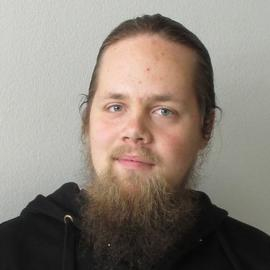
\includegraphics[width=2.1cm, trim = 0mm 0mm 0mm 0mm, clip]{Figures/OH}}\hfill%
\subcaptionbox*{Helmi Hankimaa}[.23\linewidth]{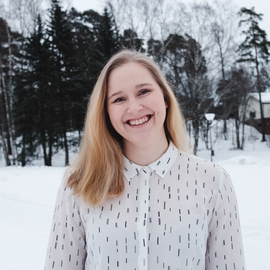
\includegraphics[width=2.3cm, trim = 0mm 0mm 0mm 10mm, clip]{Figures/HH}}\hfill%
\subcaptionbox*{Topias Terho}[.23\linewidth]{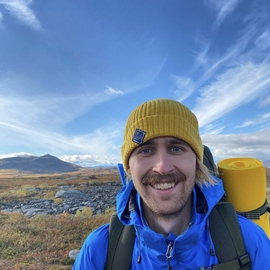
\includegraphics[width=2.3cm, trim = 20mm 0mm 0mm 20mm, clip]{Figures/TT}}\hfill%
\subcaptionbox*{Tommi Ekholm}[.3\linewidth]{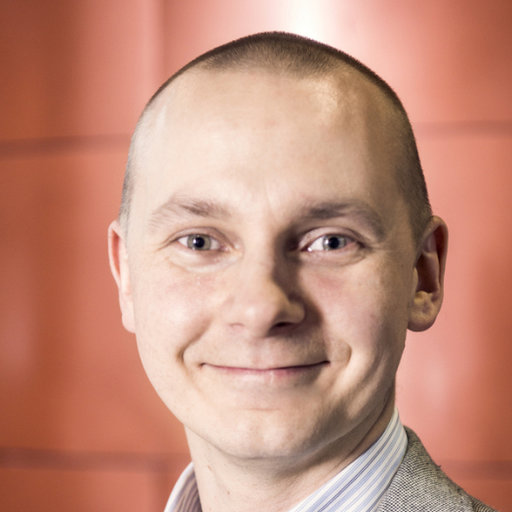
\includegraphics[width=2.2cm, trim = 0mm 0mm 0mm 10mm, clip]{Figures/TE}}\hfill%
\subcaptionbox*{Ahti Salo}[.3\linewidth]{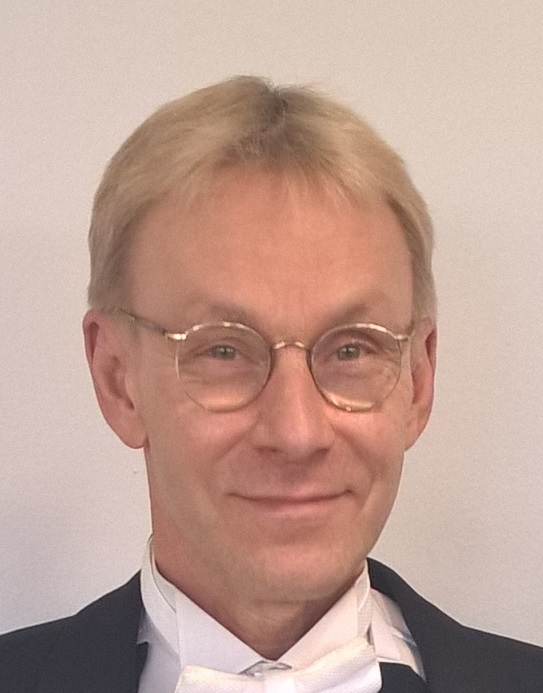
\includegraphics[width=2cm, trim = 0mm 0mm 0mm 10mm, clip]{Figures/AS.jpg}}\hfill%
\subcaptionbox*{Fabricio Oliveira}[.3\linewidth]{
\includegraphics[width=2cm, trim = 0mm 0mm 0mm 0mm, clip]{Figures/FO.jpg}}
\end{subfigure}%
\end{figure}

\end{frame}

\begin{frame}{Outline of this talk}  
\tableofcontents
\end{frame}



\section{Introduction}



\begin{frame}{Modelling decision problems}

\alert{Influence diagrams} are widely used to model decision problems under uncertainty.

\vspace{6pt}
\begin{columns}
\column{0.45\textwidth}
\begin{center}
%\setbeamercovered{invisible}
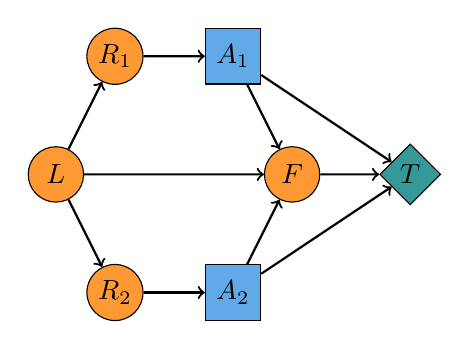
\begin{tikzpicture}
    [decision/.style={fill=blue!80, draw, minimum size=2em, inner sep=2pt}, 
    chance/.style={circle, fill=orange!80, draw, minimum size=2em, inner sep=2pt},
    value/.style={diamond, fill=teal!80, draw, minimum size=2em, inner sep=2pt},
    scale=1.5]
    %\draw[step=1cm,gray,very thin] (0,0) grid (3,2);
    \node[chance]   (L) at (0, 1)  {$L$};
    \node[chance]   (La) at (0.5, 2)  {$R_1$};
    \node[chance]   (Lb) at (0.5, 0)  {$R_2$};
    \node[decision] (A) at (1.5, 2)  {$A_1$};
    \node[decision] (B) at (1.5, 0)  {$A_2$};
    \node[chance]   (F) at (2, 1)  {$F$};
    \node[value]    (T) at (3, 1)  {$T$};     
    \draw[->, thick] (L) -- (La);
    \draw[->, thick] (L) -- (Lb);
    \draw[->, thick] (L) -- (F);
    \draw[->, thick] (La) -- (A);
    \draw[->, thick] (Lb) -- (B);
    \draw[->, thick] (A) -- (F);
    \draw[->, thick] (B) -- (F);
    \draw[->, thick] (F) -- (T);
    \draw[->, thick] (A) -- (T);
    \draw[->, thick] (B) -- (T);
\end{tikzpicture}
\end{center} 
%
\column{0.55\textwidth}
\begin{itemize}
    \item {\color{orange}Circles} denote chance events
    \item {\color{blue}Squares} denote decision events
    \item {\color{teal}Diamonds} denote value/utility calculation
    \item Arc represent \alert{influence} (dependence).
\end{itemize}

\end{columns}
\pause
\vspace{12pt}

A \alert{simple} yet \alert{powerful} tool that allows for representing a vast range of decision problems with \alert{endogenous uncertainties}. 

\end{frame}


\begin{frame}{Influence diagrams}

Despite its simplicity, obtaining solution \alert{strategies} from influence diagrams is not trivial. Methods include:
%
\begin{itemize}
    \item Form a \alert{decision tree} and solve it (backward induction);
    \item Apply arc reversal/ node elimination methods;
    \item Apply \alert{Single Policy Update} (SPU) \citep{lauritzen2001} or variant.
\end{itemize}

\pause
Influence diagrams represent \alert{Markov decision processes} and are, likewise, generally \alert{hard to solve}.
%
\begin{itemize}
    \item Solving an influence diagram is NP-Hard \citep{maua2013}
    \item Even obtaining approximate solutions is NP-Hard \citep{maua2014}
\end{itemize}
 
\end{frame}


\begin{frame}{Influence diagrams}

Moreover, several \alert{limitations} arise from relying on influence diagrams as a modelling framework:
\begin{itemize}[<+->]
    \item Solution methods require the \alert{no-forgetting} assumption: assume single decision maker or perfect information sharing.
    \item Imposing \alert{constraints} among decisions is not possible.
    \item Multiple value nodes (or objectives)
    \item Considering \alert{measures on the outcome probabilistic distribution} (e.g., chance constraints, risk measures) is not viable with traditional methods.
\end{itemize}
\onslide<+->{
{\bf Our contribution:} a framework to address the above while being computationally reliable.}

\end{frame}



\section{Decision Programming}



\begin{frame}{Decision Programming}

In specific, we propose a framework that can:
%
\begin{enumerate}
    \item exploit the \alert{expressiveness} of influence diagrams
    \item exploit \alert{linearity} (i.e., solve Mixed-Integer Linear Programs - MIPs) as opposed to \alert{recursion}. 
\end{enumerate}

\pause
In a nutshell, \alert{Decision Programming} combines:
\begin{itemize} 
    \item the structuring for decision problem under uncertainty from \alert{Decision Analysis} with 
    \item the structure of MIP formulation of deterministic equivalents for multistage \alert{Stochastic Programming} problems.
\end{itemize}


\end{frame}


\begin{frame}{Decision Programming}{Information sets and paths}

We represent an \alert{influence diagram} as an acyclic graph $G(N,A)$.
\begin{itemize}
    \item $N$ consists of chance nodes $c \in C$, decision nodes $d \in D$, and value nodes $v \in V$. Let $n = |C| + |D|$.
    \item Arcs $A = \braces{(i,j) : i,j \in N}$ represent \alert{dependencies} between nodes.
\end{itemize}

\pause
With these in mind, we define \alert{two key concepts}:
\begin{itemize}
\item {\bf Information sets:} $I(j)$ consists of nodes from which there is an arc to $j$.
\item {\bf Information states:} $s_{I(j)} \in S_{I(j)} = \prod_{i \in I(j)}S_i$ is a combination of states $s_i$ for nodes in the information set of $i \in I(j)$.
\end{itemize}

\end{frame}


\begin{frame}{Decision Programming}{Information sets and paths}

Considering the nodes $i \in C \cup D$.
\begin{itemize}[<+->]
    \item Let $X_i$ be the associated 'random' variable.
    \item {\bf At chance nodes $c \in C$:} a state $s_c$ is observed with (conditional) \alert{probability} 
    $$ \mathbb{P}(X_c = s_c \mid X_i = s_i, i \in I(c)) $$
    \item {\bf At decision nodes $d \in D$:} we define a \alert{local decision strategy} as a function $Z_d : S_{I(d)} \mapsto S_d$.
    $$ \mathbb{P}(X_d = s_d \mid X_i = s_i, i \in I(d), Z_d) = 1 \iff Z_d(s_{I(d)}) = s_d $$
\end{itemize}
%
\vspace{-24pt}
\onslide<+->{{\bf Remark:} A (global) decision strategy $Z = \prod_{d \in D} Z_d$ is the combination of all local decision strategies.}  

\end{frame}


\begin{frame}{Information sets and paths}

Another key concept: the notion of a \alert{path}.
%
\begin{itemize}
    \item Since $G$ is acyclic, $i < j$ if $(i,j) \in A$ w.l.o.g.;
    \item A {\bf path} of length $k$ is a \alert{sequence} $(s_1, s_2, \dots, s_k)$ such that $s_i \in S_i, i = 1,\dots, k$;
    \item Paths of length $n = |C| + |D|$ are denoted by 
    $$ s = (s_1, \dots, s_n) \in S = \prod_{i \in C \cup D} S_i. $$
\end{itemize}

\pause
\begin{columns}
\column{0.4\textwidth}

\vspace{-32pt}
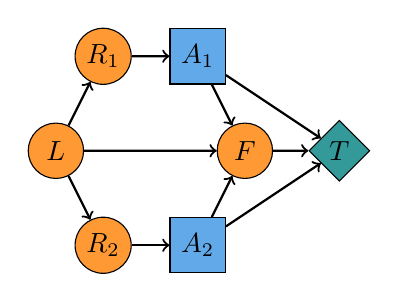
\begin{tikzpicture}
    [decision/.style={fill=blue!80, draw, minimum size=2em, inner sep=2pt}, 
    chance/.style={circle, fill=orange!80, draw, minimum size=2em, inner sep=2pt},
    value/.style={diamond, fill=teal!80, draw, minimum size=2em, inner sep=2pt},
    scale=1.2]
    %\draw[step=1cm,gray,very thin] (0,0) grid (3,2);
    \node[chance]   (L) at (0, 1)  {$L$};
    \node[chance]   (La) at (0.5, 2)  {$R_1$};
    \node[chance]   (Lb) at (0.5, 0)  {$R_2$};
    \node[decision] (A) at (1.5, 2)  {$A_1$};
    \node[decision] (B) at (1.5, 0)  {$A_2$};
    \node[chance]   (F) at (2, 1)  {$F$};
    \node[value]    (T) at (3, 1)  {$T$};     
    \draw[->, thick] (L) -- (La);
    \draw[->, thick] (L) -- (Lb);
    \draw[->, thick] (L) -- (F);
    \draw[->, thick] (La) -- (A);
    \draw[->, thick] (Lb) -- (B);
    \draw[->, thick] (A) -- (F);
    \draw[->, thick] (B) -- (F);
    \draw[->, thick] (F) -- (T);
    \draw[->, thick] (A) -- (T);
    \draw[->, thick] (B) -- (T);
\end{tikzpicture}

\column{0.6\textwidth}
{\bf Example:} assume that $L = R_1 = R_2 = ... = F = \braces{+,-}$. 
\vspace{6pt}

Then $s = (l, r_1, r_2, a_1, a_2, f) = (+, +, +, +, +, +)$ is a \alert{path}.

\end{columns}



\end{frame}


\begin{frame}{Information sets and paths}

	We can now formally state (recursively) the \alert{probability of a path given a decision strategy} $Z$
	\vspace{-12pt}
	
	{\small
	\begin{equation*} \label{path_probabilities}
	\mathbb{P}(s_{1:k}~|~Z)= \bigg( \prod_{i \in C : i \leq k} \mathbb{P} \big(X_i=s_i~|~X_{I(i)} = s_{I(i)} \big) \bigg) \bigg( \prod_{j \in D : j \leq k} \mathbb{I} \big( Z_j(s_{I(j)})=s_j \big) \bigg), 
	\end{equation*}
	}
	
	where $\mathbb{I}(\,\cdot\,)$ is defined so that 
	
	\begin{equation*}
	    \mathbb{I}(Z_j(s_{I(j)}) = s_j) = \begin{cases}1, &\text{if } Z_j(s_{I(j)})=s_j, \\
	                                       0, &\text{otherwise.} \end{cases}
	\end{equation*}

\end{frame}



\begin{frame}{Towards an MIP formulation}

	Our objective is to encode this logic into \alert{decision variables}.
	\begin{itemize}[<+->]
	\item We represent decisions with \alert{variables} $z(s_j \mid s_{I(j)}) \in \braces{0,1}$.
	%
	\begin{equation} \label{eq5}
	Z_j(s_{I(j)}) = s_j \iff z(s_j \mid s_{I(j)}) = 1, \, \forall \,j \in D,\, s_j  \in S_j, \,s_{I(j)} \in S_{I(j)}. 
	\end{equation} 
	%
	\item Mutual exclusivity implies
	%
	\begin{equation} \label{eq6}
	\sum_{s_j \in S_j} z(s_j \mid s_{I(j)}) = 1, \, \forall j \in D, s_{I(j)} \in S_{I(j)}	
	\end{equation}
	%
	\item And we define $\pi_k(s) \in [0,1]$ to represent the \alert{path probability}.
	%
	\begin{equation} \label{eq7}
	\pi_k(s) = \mathbb{P}\left(X_k = s_k \mid X_{I(k)} = s_{I(k)}\right) \pi_{k-1}(s), 
	\end{equation}
	%
	\end{itemize}
	
	\vspace{-21pt}
	\onslide<3->{
	For $k \in D$ being a decision node, we have that
	%
	\begin{equation} \label{eq8}
	\pi_k(s) = \begin{cases}
	\pi_{k-1}(s), & \quad \text{if } z(s_k \mid s_{I(k)}) = 1 \\ 
	0, & \quad \text{if } z(s_k \mid s_{I(k)}) = 0. \end{cases}  
	\end{equation}
	}
\end{frame}


\begin{frame}{Information sets and paths}

	\begin{theorem} \label{scenariopaths}
		Let $Z \in \mathbb{Z}$ be a decision strategy and choose a path $s \in S$. If $\pi_k(s)$, $k = 1, \dots, n$, and $z(s_j \mid s_{I(j)})$, $\forall j \in D$, satisfy the constraints \eqref{eq5} -- \eqref{eq8}, then 
		%
		\begin{equation*} \label{pi_recursion}
			\pi_k(s) = \mathbb{P}(X_{1:k} = s_{1:k} \mid Z), \, \forall \, k = 1,\dots,n
		\end{equation*}
		%
		In particular, $\pi(s) \overset{def}{=} \pi_n(s)$ is the probability of the path $s$ for the strategy $Z$.
	\end{theorem}

\end{frame}


\begin{frame}{Towards an MIP formulation}


	Variables $\pi_k(s)$ can be defined by the inequalities
	%
	\begin{equation*}\label{decisionconstraints}
	\text{max} \{0, \, \pi_{k-1}(s) + z(s_k \mid s_{I(k)}\textbf{}) - 1\}  \leq \pi_k(s) \leq \text{min} \{ \pi_{k-1}(s),\, z(s_k \mid s_{I(k)}) \}, 
	\end{equation*}
	%
	which are equivalent to the \alert{linear inequalities}
	%
	\begin{eqnarray}
	\pi_k(s) & \leq & \pi_{k-1}(s) \label{inequality1} \\
	\pi_k(s) & \leq & z(s_k \mid s_{I(k)}) \label{inequality2} \\
	\pi_k(s) & \geq & 0 \label{inequality3} \\
	\pi_k(s) & \geq & \pi_{k-1}(s) + z(s_k \mid s_{I(k)}) - 1. \label{inequality4}
	\end{eqnarray}

\end{frame}


\begin{frame}{Towards a MIP formulation}

	We want to maximise expected utilities using ${\cal U}:S_{I(v)} \to \mathbb{R}$.
	%
	\begin{equation*}
	\text{max.}_{Z \in \mathbb{Z}} \sum_{s \in S} \pi_n(s) {\cal U}(s)
	\end{equation*}
	%
	which only involve $\pi_n(s) = \pi(s)$. \pause Notice that these can be \alert{pre-calculated for any given strategy $Z \in \mathbb{Z}$.}
	%
	\begin{equation*}
	p(s) = \prod_{j \in C} \mathbb{P}(X_j = s_j \mid X_{I(j)} = s_{I(j)}).
	\end{equation*}
	%
	And then 
	\vspace{-6pt}
	\begin{itemize}
	\item if $Z$ is \alert{compatible} with $s \in S$ (i.e., if $Z$ maps to path $s \in S$), then $\pi(s) = p(s)$
	\item otherwise, $\pi(s) = 0$.
	\end{itemize}

\end{frame}



\begin{frame}{Towards an MIP formulation}

\vspace{6pt}

\begin{corollary}\label{cor:opt1}
	The expected utility is maximised by the strategy $Z\in \mathbb{Z}$ which solves the optimisation problem  
	%
	\vspace{-3pt}
	\begin{equation*}\label{optimization} \small
		\maxi_{Z \in \mathbb{Z}} \sum_{s \in S} \pi(s) \mathcal{U}(s)
	\end{equation*}
		
	subject to constraints \eqref{eq5} -- \eqref{eq7} and \eqref{inequality1} -- \eqref{inequality4} on decision variables $z(s_k|s_{I(k)}) \in \{0,1\}, \, \forall k \in D$, $s_k \in S_k, s_{I(k)} \in S_{I(k)}$ and path probabilities $\pi_k(s) \in [0,1], \forall s \in S$.    
\end{corollary}

\vspace{-6pt}
\pause	
The formulation \alert{recursively simplified} to only consider $k=n$, since
\vspace{-6pt}
\begin{itemize}
	\item \eqref{inequality1} -- \eqref{inequality4} imply that $\pi_j(s) = \pi_{j-1}(s)$ for each $j \in D$ if $z(s_j \mid s_{I(j)}) = 1$
	\item Analogously, if the strategy $Z$ is not compatible with $s$, $\pi_n(s) \leq \pi_j(s) = 0$ if $z(s_j \mid s_{I(j)}) = 0$ for some $j \in D$.
\end{itemize}
	
	
\end{frame}




\begin{frame}{Towards a MIP formulation}

The complete formulation is given by
%
{\small
\begin{align*}
& \text{max.}_{Z \in \mathbb{Z}} ~~  \sum_{s \in S} \pi(s) {\cal U}(s) \\
& \text{s.t.:}  \\
~~\, & \sum_{s_j \in S_j} z(s_j \mid s_{I(j)}) = 1, &&\forall \,j \in D, s_{I(j)} \in S_{I(j)} \\ 
& 0 \leq \pi(s) \leq p(s),  && \forall\, s \in S \\
& \pi(s) \leq z(s_j \mid s_{I(j)}), &&\forall\, j \in D , s\in S \\
& \pi(s) \geq p(s) + \sum_{j \in D} z(s_j \mid s_{I(j)}) - |D|,  &&\forall\, s \in S \\ 
& z(s_j \mid s_{I(j)}) \in \{0,1\}, &&\forall\, j \in D,\, s_j \in S_j, \, s_{I(j)} \in S_{I(j)}. 
\end{align*}
}
%
\end{frame}


\begin{frame}{MIP formulation: key features}

Some points worth highlighting:
\begin{enumerate}[<+->]
\item Notice that utilities ${\cal U}(s)$ and probabilities $p(s)$ can be (efficiently) computed \alert{beforehand}.
\item We tried to linearise the product of variables in  
$$\pi_k(s) = \mathbb{P}\left(X_k = s_k \mid X_{I(k)} = s_{I(k)}\right) \pi_{k-1}(s), $$
but the formulation obtained was weaker (in terms of LP relaxation).
\item The model has \alert{exploitable structure}. For example, we use (as lazy constraints) \alert{probability cuts} of the form
$$\sum_{s\in S} \pi(s) = 1.$$
\end{enumerate}

\end{frame}


%\begin{frame}{MIP formulation: example}
%
%For the 2-monitoring example we obtain:
%\vspace{12pt}
%\begin{columns}
%\column{0.5\textwidth}
%\begin{tikzpicture}
%    [decision/.style={fill=blue!80, draw, minimum size=2em, inner sep=2pt}, 
%    chance/.style={circle, fill=orange!80, draw, minimum size=2em, inner sep=2pt},
%    value/.style={diamond, fill=teal!80, draw, minimum size=2em, inner sep=2pt},
%    scale=1.5]
%    %\draw[step=1cm,gray,very thin] (0,0) grid (3,2);
%    \node[chance]   (L) at (0, 1)  {$L$};
%    \node[chance]   (La) at (0.5, 2)  {$R_1$};
%    \node[chance]   (Lb) at (0.5, 0)  {$R_2$};
%    \node[decision] (A) at (1.5, 2)  {$A_1$};
%    \node[decision] (B) at (1.5, 0)  {$A_2$};
%    \node[chance]   (F) at (2, 1)  {$F$};
%    \node[value]    (T) at (3, 1)  {$T$};     
%    \draw[->, thick] (L) -- (La);
%    \draw[->, thick] (L) -- (Lb);
%    \draw[->, thick] (L) -- (F);
%    \draw[->, thick] (La) -- (A);
%    \draw[->, thick] (Lb) -- (B);
%    \draw[->, thick] (A) -- (F);
%    \draw[->, thick] (B) -- (F);
%    \draw[->, thick] (F) -- (T);
%    \draw[->, thick] (A) -- (T);
%    \draw[->, thick] (B) -- (T);
%\end{tikzpicture}
%
%\column{0.5\textwidth}
%
%The nodes are
%\begin{itemize}
%\item $C = \{ L,R^1, R^2, F \}$, 
%\item $D = \{ A^1,A^2 \}$
%\end{itemize}
%The \alert{information structure}:
%\begin{itemize}
%\item $I(R^i) = \{ L \}, i=1,2$, 
%\item $I(A^i) = \{ R^i \}, i=1,2$
%\item $I(F)= \{L,A^1, A^2\}$
%\item $I(T) = \{ A^1,A^2, F \}$
%\end{itemize}
%
%\end{columns}
%\pause
%An order satisfying the information structure: $$s = (l,r^1,r^2,a^1,a^2,f).$$
%
%\end{frame}
%
%
%\begin{frame}{MIP formulation: example}
%
%For the 2-monitoring example we obtain:
%%
%{\footnotesize
%\begin{align*}
%\mathop{\text{max.}}\limits_{Z \in \mathbb{Z}} ~~&\sum_{(l,r_1,r_2,a_1,a_2,f)} \pi(l,r_1,r_2,a_1,a_2,f) U\big[Y_T(a_1,a_2,f)\big] \\
%\text{s.t.:} ~\, & \sum_{a_i} z(a_i \mid r_i) = 1, && \forall \, r_i \in R_i,  i=1,2 \\
%& 0 \leq \pi(l,r_1,r_2,a_1,a_2,f) \leq  p(l,r_1,r_2,a_1,a_2,f), && \forall \, (l,r_1,r_2,a_1,a_2,f)  \\
%& \pi(l,r_1,r_2,a_1,a_2,f) \leq z(a_i \mid r_i), && \forall \, (l,r_1,r_2,a_1,a_2,f), i=1,2 \\
%& \pi(l,r_1,r_2,a_1,a_2,f) \geq \\
%& \quad p(l,r_1,r_2,a_1,a_2,f) + \sum_{i=1,2}z(a_i \mid r_i) - 2, && \forall \, (l,r_1,r_2,a_1,a_2,f) \\
%& z(a_i \mid r_i) \in \{0,1\}, && \forall \, r_i \in R_i,  i=1,2.
%\end{align*}
%}
%%
%where $Y_T(a_1,a_2,f)$ gives the consequences associated with the failure state $F = f$ and the actions $A^1 = a_1$ and $A^2 = a_2$.
%\end{frame}


%\begin{frame}{MIP formulation: example}
%
%\begin{center}
%\huge
%{\color{blue}EXCEL Example}
%\end{center}
%
%
%
%\end{frame}



\section{Computational experiments}


\begin{frame}{Examples}{N-monitoring problem}

%A stylised problem where the no-forgetting assumption doesn't hold: no decision tree formulation is possible.

N agents independently intervening without sharing information.

\begin{columns}

\column{0.4\textwidth}
\begin{itemize}
\item \alert{Independent} parallel measures;
\item Decisions that can't be communicated;
\item \alert{No no-forgetting}: each action can be seen as taken by independent decision makers.
\end{itemize}

\column{0.6\textwidth}
\begin{center}
%\setbeamercovered{invisible}
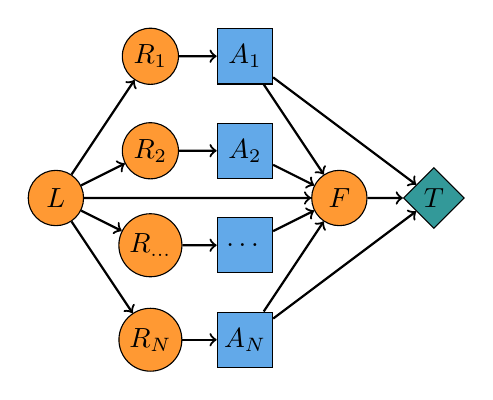
\begin{tikzpicture}
    [decision/.style={fill=blue!80, draw, minimum size=2em, inner sep=2pt}, 
    chance/.style={circle, fill=orange!80, draw, minimum size=2em, inner sep=2pt},
    value/.style={diamond, fill=teal!80, draw, minimum size=2em, inner sep=2pt},
    scale=1.2]
    %\draw[step=1cm,gray,very thin] (0,0) grid (4,3);
    \node[chance]   (L) at (-0.25, 1.5)  {$L$};
    \node[chance]   (L1) at (0.75, 3)  {$R_1$};
    \node[chance]   (L2) at (0.75, 2)  {$R_2$};
    \node[chance]   (LN-1) at (0.75, 1)  {$R_{\dots}$};
    \node[chance]   (LN) at (0.75, 0)  {$R_N$};
    \node[decision] (1) at (1.75, 3)  {$A_1$};
    \node[decision] (2) at (1.75, 2)  {$A_2$};
    \node[decision] (N-1) at (1.75, 1)  {$\dots$};
    \node[decision] (N) at (1.75, 0)  {$A_N$};
    \node[chance]   (F) at (2.75, 1.5)  {$F$};
    \node[value]    (T) at (3.75, 1.5)  {$T$};     
    \draw[->, thick] (L) -- (L1);
    \draw[->, thick] (L) -- (L2);
    \draw[->, thick] (L) -- (LN-1);
    \draw[->, thick] (L) -- (LN);
    \draw[->, thick] (L) -- (F);
    \draw[->, thick] (L1) -- (1);
    \draw[->, thick] (L2) -- (2);
    \draw[->, thick] (LN-1) -- (N-1);
    \draw[->, thick] (LN) -- (N);
    \draw[->, thick] (1) -- (F);
    \draw[->, thick] (2) -- (F);
    \draw[->, thick] (N-1) -- (F);
    \draw[->, thick] (N) -- (F);
    \draw[->, thick] (F) -- (T);
    \draw[->, thick] (1) -- (T);
    \draw[->, thick] (N) -- (T);
\end{tikzpicture}
\end{center}

\end{columns}
\pause
{\bf Remark:} can be shown to not be \alert{soluble} \citep{lauritzen2001}, a sufficient condition for SPU to converge to optimal strategies.

\end{frame}


\begin{frame}{Computational experiments\footnote{\tiny{\bf Computational setting:} Intel Xeon E3-1230 @ 3.40 GHz with 32 GB RAM; coded in Julia 1.1.0 (JuMP 0.18.6); solved with Gurobi 8.1.0.}}{N-monitoring problem}  
%
{\small
\begin{table}[htp!] %{tab:n-m_solution_time}
	\centering
	\setlength{\tabcolsep}{1.0pt}
	{\footnotesize{
\begin{tabular}{c@{\extracolsep{15pt}}c@{\extracolsep{0pt}}r@{\extracolsep{15pt}}r@{\extracolsep{0pt}}r@{\extracolsep{15pt}}r@{\extracolsep{0pt}}r}
\toprule
\multicolumn{1}{l}{} & 
\multicolumn{2}{c}{Number of variables} &
\multicolumn{2}{c}{No probability cuts} &
\multicolumn{2}{c}{With probability cuts} \\
\cmidrule{2-3}
\cmidrule{4-5}
\cmidrule{6-7}
\multicolumn{1}{l}{\# Nodes} &
\multicolumn{1}{r}{Binary} &
\multicolumn{1}{r}{Real} &
\multicolumn{1}{r}{A} & 
\multicolumn{1}{r}{SD} & 
\multicolumn{1}{r}{A} & 
\multicolumn{1}{r}{SD}\\
\midrule
2  &  \p{1}8  &   64~~  &	    0.01 	&	 0.01   &	   0.01 	&	  0.00 \\
3  & 12  &     256~~  &	    0.12 	&	 0.08 	&	   0.02 	&	  0.01 \\
4  & 16  &    1~024~~  &	    0.79 	&    0.53	&      0.07 	&	  0.02 \\
5  & 20  &    4~096~~  &     5.94 	&    2.80   &      0.35  	&	  0.19 \\
6  & 24  &   16~384~~  &    77.35    &   46.31  	&	   2.44 	&	  1.63 \\
7  & 28  &   65~536~~  &   676.35    &  468.09  	&     20.58 	&    17.48 \\
8  & 32  &  262~144~~  &	8~474.00 & 7~377.28  &	 268.93 	&	330.89 \\
9  & 36  & 1~048~576~~  & 	  -      &	 	-    &   1~727.19    &  2~880.20 \\
%10	&	 	&	 	&	 	&	 		\\
\bottomrule
\end{tabular}
}}
	\caption{Solution times (s) for 10 randomly generated instances.}\label{tab:n-m_solution_time}
\end{table}
}


	
\end{frame}


\begin{frame}{Examples}{Pig farm problem}

The original problem introducing LIMID as not soluble.

\begin{columns}

\column{0.55\textwidth}

\begin{figure}
\centering 

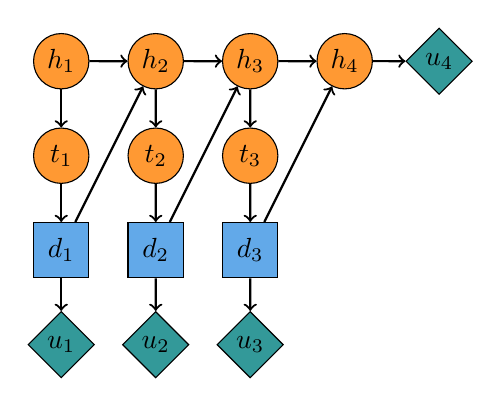
\begin{tikzpicture}
    [decision/.style={fill=blue!80, draw, minimum size=2em, inner sep=2pt}, 
    chance/.style={circle, fill=orange!80, draw, minimum size=2em, inner sep=2pt},
    value/.style={diamond, fill=teal!80, draw, minimum size=2em, inner sep=2pt},
    scale=1.2]
     %\draw[step=1cm,gray,very thin] (0,0) grid (4,3);
     \node[chance] (h1) at (0, 3)      {$h_1$};
     \node[chance] (h2) at (1, 3)      {$h_2$};
     \node[chance] (h3) at (2, 3)      {$h_3$};
     \node[chance] (h4) at (3, 3)      {$h_4$};
     \node[value]  (u4) at (4, 3)      {$u_4$};
     \node[chance] (t1) at (0, 2)      {$t_1$};
     \node[chance] (t2) at (1, 2)      {$t_2$};
     \node[chance] (t3) at (2, 2)      {$t_3$};
     \node[decision] (d1) at (0, 1)    {$d_1$};
     \node[decision] (d2) at (1, 1)    {$d_2$};
     \node[decision] (d3) at (2, 1)    {$d_3$};
     \node[value] (u1) at (0, 0)       {$u_1$};
     \node[value] (u2) at (1, 0)       {$u_2$};
     \node[value] (u3) at (2, 0)       {$u_3$};
     \draw[->, thick] (h1) -- (t1);
     \draw[->, thick] (h1) -- (h2);
     \draw[->, thick] (h2) -- (t2);
     \draw[->, thick] (h2) -- (h3);
     \draw[->, thick] (h3) -- (t3);
     \draw[->, thick] (h3) -- (h4);
     \draw[->, thick] (h4) -- (u4);
     \draw[->, thick] (t1) -- (d1);
     %\draw[->, thick] (t1) -- (d2);
     %\draw[->, thick] (t1) -- (d3);
     \draw[->, thick] (t2) -- (d2);
     %\draw[->, thick] (t2) -- (d3);
     \draw[->, thick] (t3) -- (d3);
     %\draw[->, thick] (d1) -- (d2);
     \draw[->, thick] (d1) -- (h2);
     \draw[->, thick] (d1) -- (u1);
     \draw[->, thick] (d2) -- (h3);
     \draw[->, thick] (d2) -- (u2);
     %\draw[->, thick] (d2) -- (d3);
     %\draw[->, thick] (d1) -- (0.5, 0.5) -- (1.5,0.5) -- (d3);
     \draw[->, thick] (d3) -- (h4);
     \draw[->, thick] (d3) -- (u3);
\end{tikzpicture}
\caption{The pig farm problem with 4 periods \citep{lauritzen2001}.} \label{FigurePigs}
\end{figure}


\column{0.45\textwidth}
\vspace{-25pt}
\begin{itemize}
	\item Each month pigs are tested for a disease
	\item Decide whether to inject curative/preventive drug.	
	\item Sick pigs worth less at the end.
	\item No record is kept for individual pigs.	
\end{itemize}

	
\end{columns}



\end{frame}


\begin{frame}{Computational experiments\footnote{\tiny{\bf Computational setting:} Intel Xeon E3-1230 @ 3.40 GHz with 32 GB RAM; coded in Julia 1.1.0 (JuMP 0.18.6); solved with Gurobi 8.1.0.}}{Pig farm problem}

Obtaining \alert{optimal} solutions is fairly easy.

\begin{table}[htp!]
	\centering
	\label{tab:pigs_solutions}
	\setlength{\tabcolsep}{5.0pt}
	{\footnotesize{
\begin{tabular}{ccc}

\toprule

\# Months & Optimal value (DKK) & Solution time (s) \\ 
\midrule
3	& 764 & \p{00}0.01 \\
4	& 727 & \p{00}0.04 \\
5	& 703 & \p{00}0.62 \\
6	& 686 & \p{0}19.52  \\
7   & 674 & 617.21\\
\bottomrule
\end{tabular}
}}
\caption{Results for the pig farm problem for different numbers of periods.}
\end{table}
\pause
%
\vspace{-16pt}
We extend the example incorporating \alert{risk aversion} (CVaR) and calculating all \alert{non-dominated strategies}, originally not possible.

\end{frame}


\begin{frame}{Extra: Pig farm problem with risk considerations}

\centering

\begin{figure}
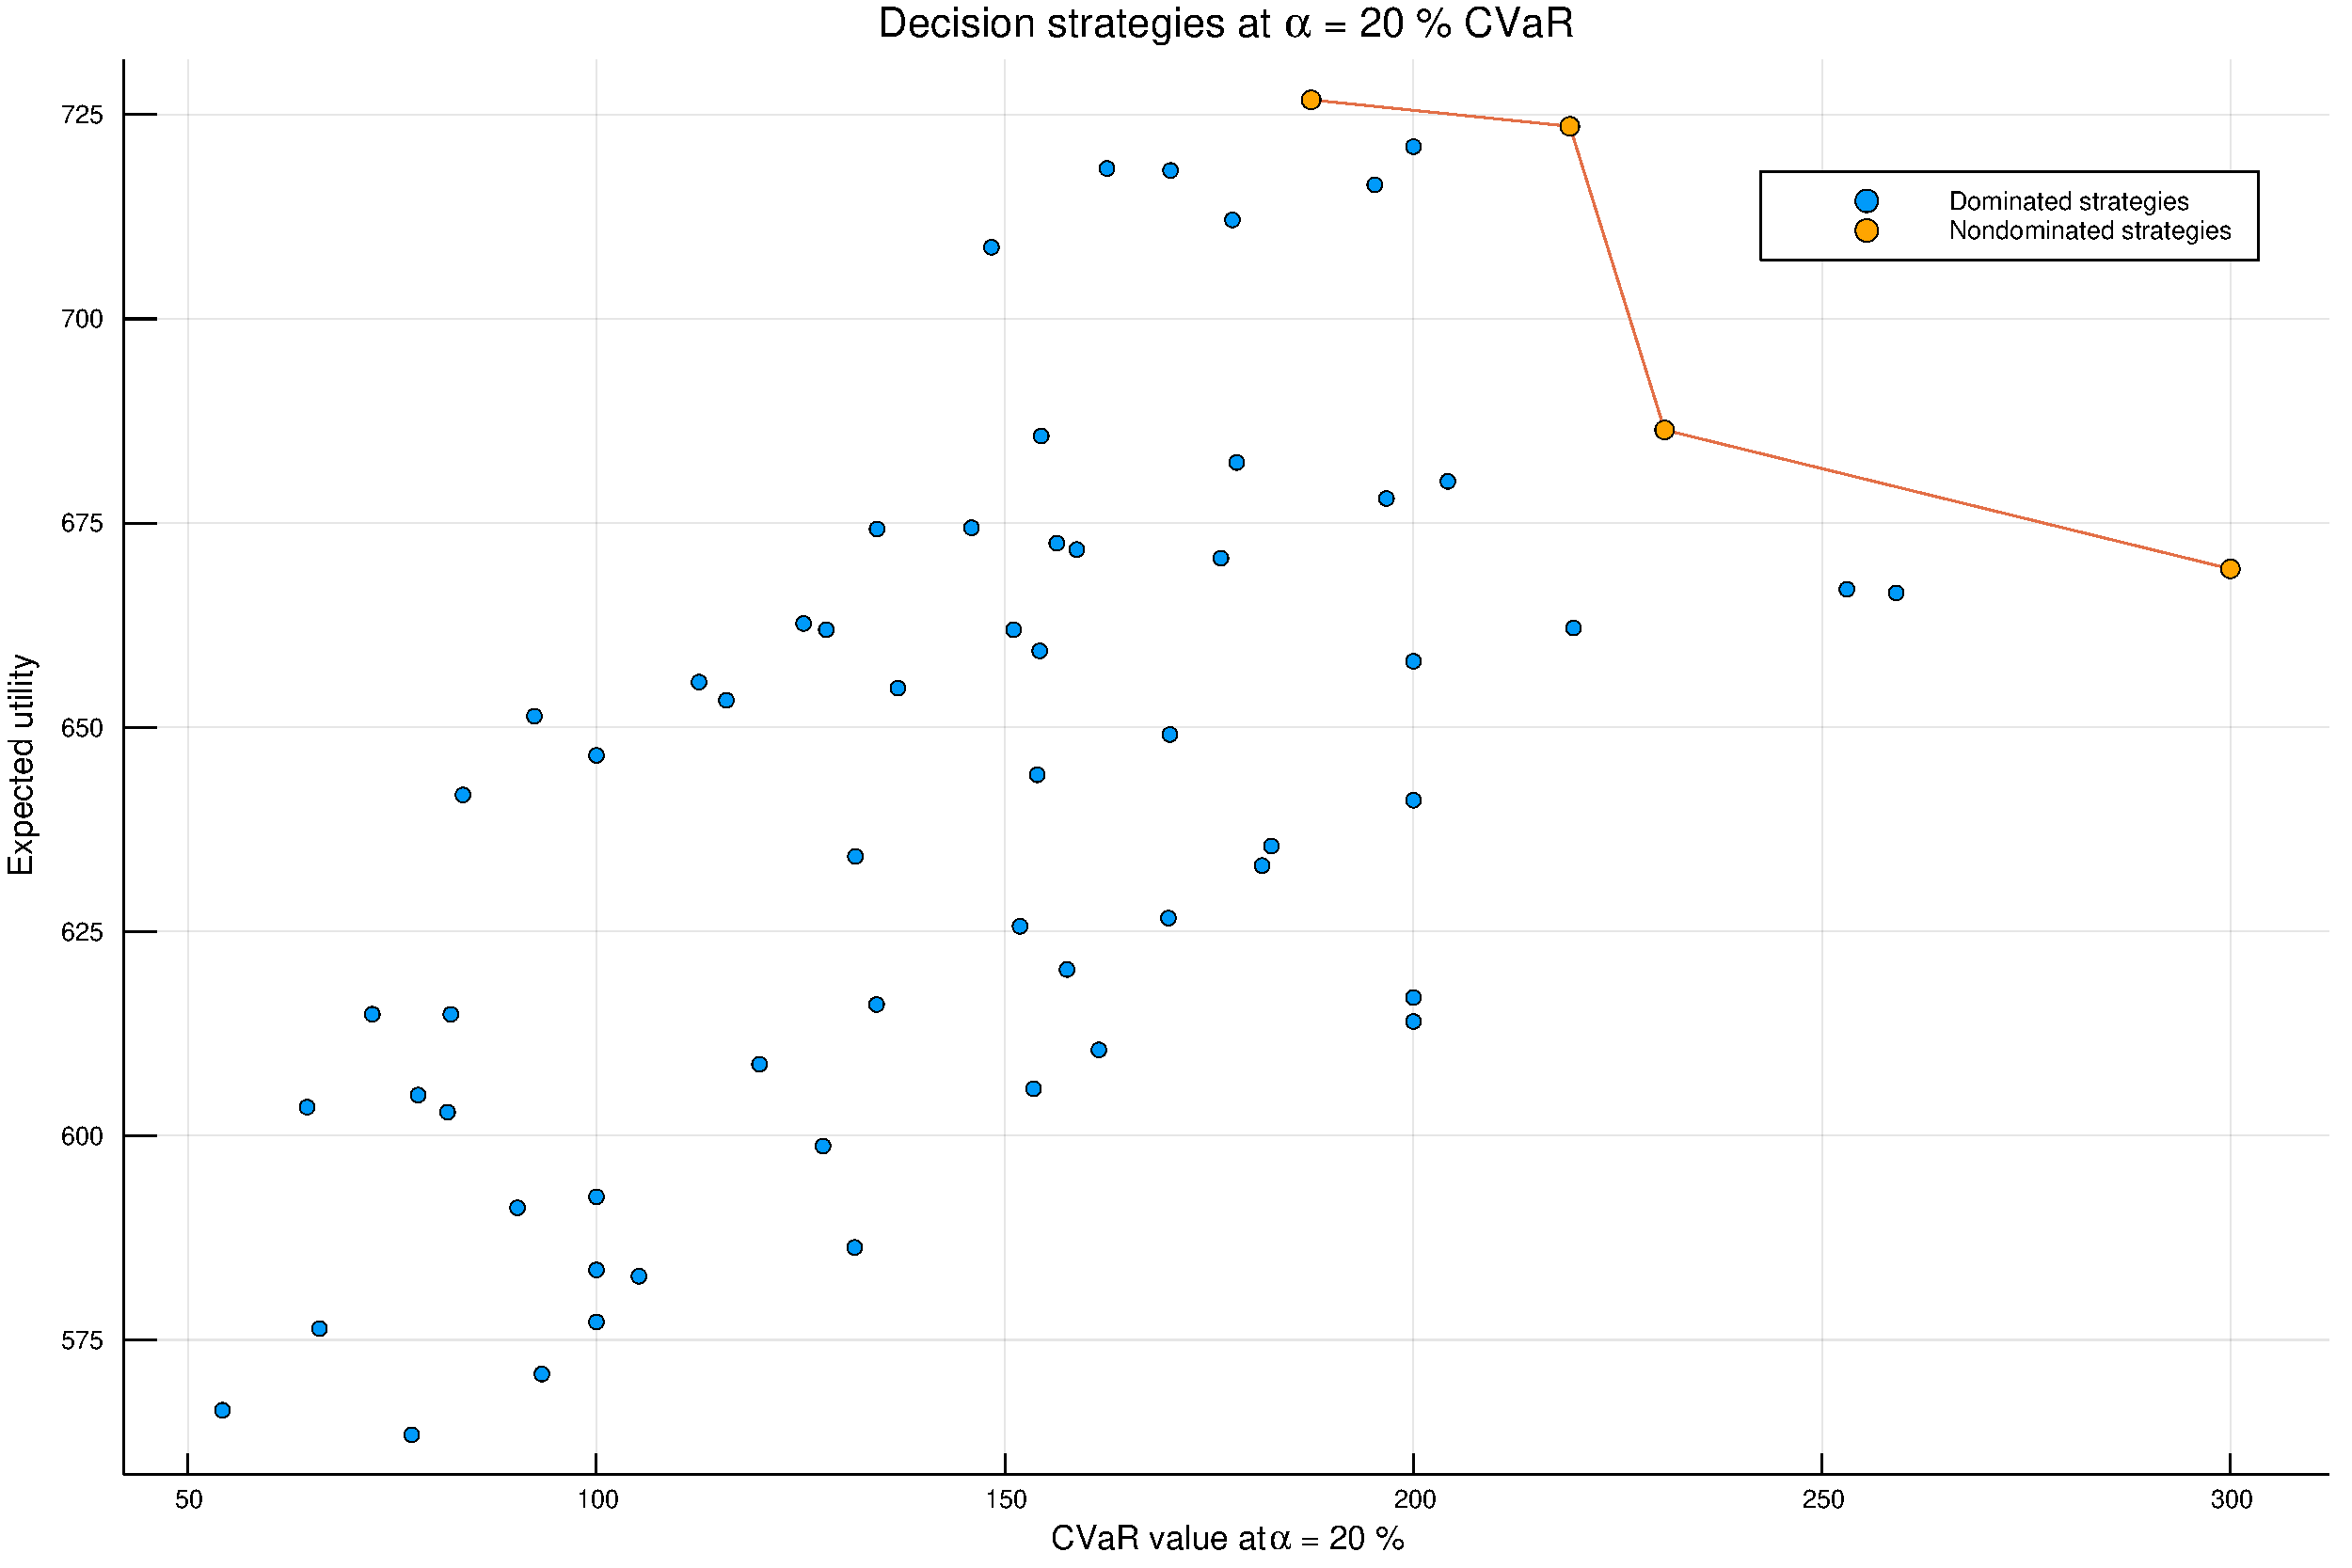
\includegraphics[width = 0.75\textwidth]{Figures/plot_cvar_util.pdf}
\caption{\footnotesize Expected utilities and conditional expectations in the lower $\alpha = 0.20$ tail for all 64 strategies of the 4-month pig problem.}
\label{fig:cvar_pigs}
\end{figure}
	
\end{frame}




%\begin{frame}{ECP-selection problem}
%
%An \alert{endogenously uncertain} portfolio selection problem. 
%
%\begin{columns}
%
%\column{0.4\textwidth}
%\begin{itemize}
%\item Select portfolio of actions to maximise expected benefit.
%\item The probability distribution of the outcomes is affected by decisions
%\item Likewise, outcomes could be affected.
%\end{itemize}
%
%
%\column{0.6\textwidth}
%
%\begin{center}
%%\setbeamercovered{invisible}
%\begin{tikzpicture}
%    [decision/.style={fill=blue!80, draw, minimum size=2em, inner sep=2pt}, 
%    chance/.style={circle, fill=orange!80, draw, minimum size=2em, inner sep=2pt},
%    value/.style={diamond, fill=teal!80, draw, minimum size=2em, inner sep=2pt},
%    scale=1.3]
%    %\draw[step=1cm,gray,very thin] (0,0) grid (4,3);
%     \node[chance] (I) at (0, 1.5)     {$I$};
%     \node[decision] (As) at (0.5, 2.5)    {$A_s$};
%     \node[decision] (Ac) at (2, 2.5)    {$A_c$};          
%     \node[decision] (Bs) at (0.5, 0.5)    {$B_s$};
%     \node[decision] (Bc) at (2, 0.5)    {$B_c$};
%     \node[chance]   (S1) at (1, 1.5)  {$C_1$};
%     \node[chance]   (S2) at (2.5, 1.5)  {$C_2$};
%     \node[value]    (VA) at (3.5, 2.5)    {$V_A$};
%     \node[value]    (V)  at (4, 1.5) {$V$};                     
%     \node[value]    (VB) at (3.5, 0.5)    {$V_B$};
%     \draw[->, thick] (I) -- (As);
%     \draw[->, thick] (I) -- (Bs);
%     \draw[->, thick] (As) -- (Ac);
%     \draw[->, thick] (As) -- (0.5, 3.25) -- (3.5, 3.25) -- (VA);
%     \draw[->, thick] (Bs) -- (0.5, -0.25) -- (3.5, -0.25) -- (VB);
%     \draw[->, thick] (Bs) -- (Bc);
%     \draw[->, thick] (Ac) -- (VA);
%     \draw[->, thick] (Bc) -- (VB);
%     \draw[->, thick] (S1) -- (Ac);
%     \draw[->, thick] (S1) -- (I);
%     \draw[->, thick] (S1) -- (Bc);
%     \draw[->, thick] (S1) -- (VA);
%     \draw[->, thick] (S1) -- (VB);
%     \draw[->, thick] (Ac) -- (S2);
%     \draw[->, thick] (Bc) -- (S2);
%     \draw[->, thick] (VA) -- (V);
%     \draw[->, thick] (VB) -- (V);
%     \draw[->, thick] (S2) -- (V);
%\end{tikzpicture}
%\end{center}
%
%\end{columns}
%
%Can be seen as a generalisation of \citet{gustafsson2005} for to consider the endogenous case.
%
%
%\end{frame}


%\begin{frame}{Computational experiments\footnote{{\bf Computational setting:} Intel Xeon E3-1230 @ 3.40 GHz with 32 GB RAM; coded in Julia 1.1.0 (JuMP 0.18.6); solved with Gurobi 8.1.0.}} 
%
%{\small
%\begin{table}[htp!]
%	\centering
%	\setlength{\tabcolsep}{4.0pt}
%	{\footnotesize{
%\begin{tabular}{l@{\extracolsep{15pt}}c@{\extracolsep{10pt}}r@{\extracolsep{15pt}}c@{\extracolsep{10pt}}cr}
%\toprule
%\multicolumn{1}{l}{} & \multicolumn{2}{c}{With probability cuts} & \multicolumn{3}{c}{Without probability cuts} \\
%\cmidrule{2-3}
%\cmidrule{4-6}
%\multicolumn{1}{l}{Instance} & \multicolumn{1}{c}{Solution} & \multicolumn{1}{c}{Time (s)} &
%\multicolumn{1}{c}{Solution} & \multicolumn{1}{c}{Time $(s)$} & \multicolumn{1}{c}{\%opt}\\
%\midrule
%7M1	&	73.21	&	77~~~~~~	&	73.21	&	21795	&	0.00	\\
%7M2	&	79.58	&	60~~~~~~	&	79.58	&	24951	&	0.00	\\
%7M3	&	67.84	&  105~~~~~~	&	67.84	&	13318	&	0.00	\\
%7M4	&	70.25	&  216~~~~~~	&	70.25	&	23464	&	0.00	\\
%7M5	&	62.48	&  101~~~~~~	&	62.48	&	18865	&	0.00	\\
%7M6	&	64.61	&  136~~~~~~	&	64.61	&	20787	&	0.00	\\
%7M7	&	60.57	&  110~~~~~~	&	60.57	&	11597	&	0.00	\\
%7M8	&	81.75	&	61~~~~~~	&	81.75	&	20531	&	0.00	\\
%7M9	&	79.50	&	78~~~~~~	&	79.50	&	17329	&	0.00	\\
%7M10&	69.41	&  186~~~~~~	&	69.41	&	22044	&	0.00	\\
%\midrule
%Average	&	70.92	&	113~~~~~~	&	70.92	&	19468	&	0.00	\\
%\bottomrule
%\end{tabular}
%}}
%\caption{10 randomly generated 7-monitoring instances. 65,536 paths.}\label{tab:7M}
%\end{table}
%}
%
%\end{frame}
%
%
%\begin{frame}{Computational experiments\footnote{{\bf Computational setting:} Intel Xeon E3-1230 @ 3.40 GHz with 32 GB RAM; coded in Julia 1.1.0 (JuMP 0.18.6); solved with Gurobi 8.1.0.}} 
%\vspace{-12pt}
%\begin{table}[htp!]
%	\centering
%	\setlength{\tabcolsep}{4.0pt}
%	{\footnotesize{
%\begin{tabular}{l@{\extracolsep{15pt}}c@{\extracolsep{10pt}}r@{\extracolsep{15pt}}c@{\extracolsep{10pt}}cr}
%\toprule
%\multicolumn{1}{l}{} & \multicolumn{2}{c}{With probability cuts} & \multicolumn{3}{c}{Without probability cuts} \\
%\cmidrule{2-3}
%\cmidrule{4-6}
%\multicolumn{1}{l}{Instance} & \multicolumn{1}{c}{Solution} & \multicolumn{1}{c}{Time (s)} &
%\multicolumn{1}{c}{Solution} & \multicolumn{1}{c}{Time $(s)$} & \multicolumn{1}{c}{\%opt}\\
%\midrule
%8M1	&	65.10	&	1776~~~~~	&	27.86	&	25200	&	11260.89~	\\
%8M2	&	75.34	&	2099~~~~~	&	50.28	&	25200	&	7863.56~	\\
%8M3	&	78.75	&	1090~~~~~	&	46.27	&	25200	&	7033.49~	\\
%8M4	&	73.59	&	1122~~~~~	&	73.59	&	25200	&	4962.71~	\\
%8M5	&	55.67	&	2458~~~~~	&	34.36	&	25200	&	8092.27~	\\
%8M6	&	78.68	&	1689~~~~~	&	78.53	&	25200	&	5515.04~	\\
%8M7	&	70.59	&	1714~~~~~	&	7.73	&	25200	&	49966.90~	\\
%8M8	&	82.67	&	 643~~~~~	&	13.27	&	25200	&	24215.28~	\\
%8M9	&	75.17	&	1356~~~~~	&	60.01	&	25200	&	5543.61~	\\
%8M10&	73.33	&	 879~~~~~	&	71.03	&	25200	&	4767.88~	\\
%\midrule
%Average	&	72.89	&	1483~~~~~	&	46.29	&	25200	&	12922.16~	\\
%\bottomrule
%\end{tabular}
%}}
%\caption{10 randomly generated 8-monitoring instances. 262,144 paths.}\label{tab:7M}
%\end{table}
%
%
%\end{frame}


\section{Conclusions}


\begin{frame}{Key points and takeaways}
%
\begin{center}
{\bf Decision Programming = 

\alert{Decision} Analysis + Mathematical \alert{Programming}}
\end{center}
\pause
\begin{itemize}
\item Decision Programming exploits \alert{linearity instead of recursion} to solve decision diagrams.
\item Pre-calculating the path probabilities $p(s)$ and utilities ${\cal U}$ \linebreak can be \alert{done efficiently} (in parallel).   
\item Mathematical programming as underpinning framework \linebreak allows for flexibility in terms of \alert{imposing constraints}.
\item ``Future'' work: modelling endogenously uncertain problems and solution methods (preprocessing and heuristics). 
\end{itemize}

\end{frame}


\begin{frame}{To learn more:}

\large

{\bf Main reference: } Salo et al. (2022), Decision programming for multi-stage optimization under uncertainty, EJOR, 299 (2), 550-565. DOI: \href{https://doi.org/10.1016/j.ejor.2021.12.013}{\alert{10.1016/j.ejor.2021.12.013}}

\vfill


{{\bf Julia package with many other examples:} \href{https://github.com/gamma-opt/DecisionProgramming.jl}{\alert{github.com/gamma-opt/DecisionProgramming.jl}}} 

{\bf Some newer WiP:} 
\\
{\small
Andelmin, Juho, et al. "DecisionProgramming.jl - A framework for modelling decision problems using mathematical programming." arXiv preprint \href{https://arxiv.org/abs/2307.13299}{\alert{arXiv:2307.13299}} (2023).}

{\small
Herrala, Olli, Tommi Ekholm, and Fabricio Oliveira. "A decomposition strategy for decision problems with endogenous uncertainty using mixed-integer programming." arXiv preprint \href{https://arxiv.org/abs/arXiv:2304.02338}{\alert{arXiv:2304.02338}} (2023).}

\end{frame}

\section{Recent developments}

\begin{frame}{More recent developments}

{\bf 1. Modelling long-term endogenous climate uncertainty}
\vspace{-6pt}
\begin{itemize}
	\item Consider decision-dependent (endogenous) uncertainties
	\item Take into account continuous decision spaces
\end{itemize}

We develop the notions of \alert{extended value node}
\begin{equation*}
    U_v(s_{I(v)}) := \text{max.}_y \{f_{s_{I(v)}}(y) \mid y \in Y_{s_{I(v)}}\}, \text{ for } v \in V,
\end{equation*} 
%
and \alert{conditional arcs}
\vspace{-12pt}
\begin{center}
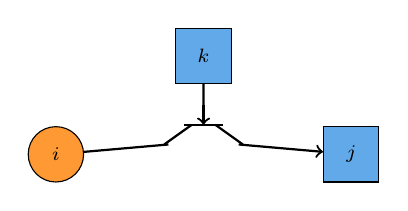
\begin{tikzpicture}
    [decision/.style={fill=blue!80, draw, minimum size=2em, inner sep=2pt}, 
    chance/.style={circle, fill=orange!80, draw, minimum size=2em, inner sep=2pt},
    value/.style={diamond, fill=teal!80, draw, minimum size=2em, inner sep=2pt},
    optimization/.style={ellipse, fill=teal!80, draw, minimum size=2em, inner sep=2pt},
    scale=1.25, font=\scriptsize]
    \node[chance] (C1) at (0, 0)        {$i$};
    \node[decision] (D1) at (1.5,1)      {$k$};
    \node[decision] (D2) at (3, 0)        {$j$};
    \draw[] (1.5,0.1) pic{dist_arc={int1, , ,}};
    \draw[thick] (C1) -- (int1.west);
    \draw[thick] (D1) --  (int1.north);
    \draw[->, thick] (int1.east) --  (D2);
\end{tikzpicture}	
\end{center}

\end{frame}

\begin{frame}{Climate change mitigation}
	\vspace{-9pt}
	\begin{figure}
	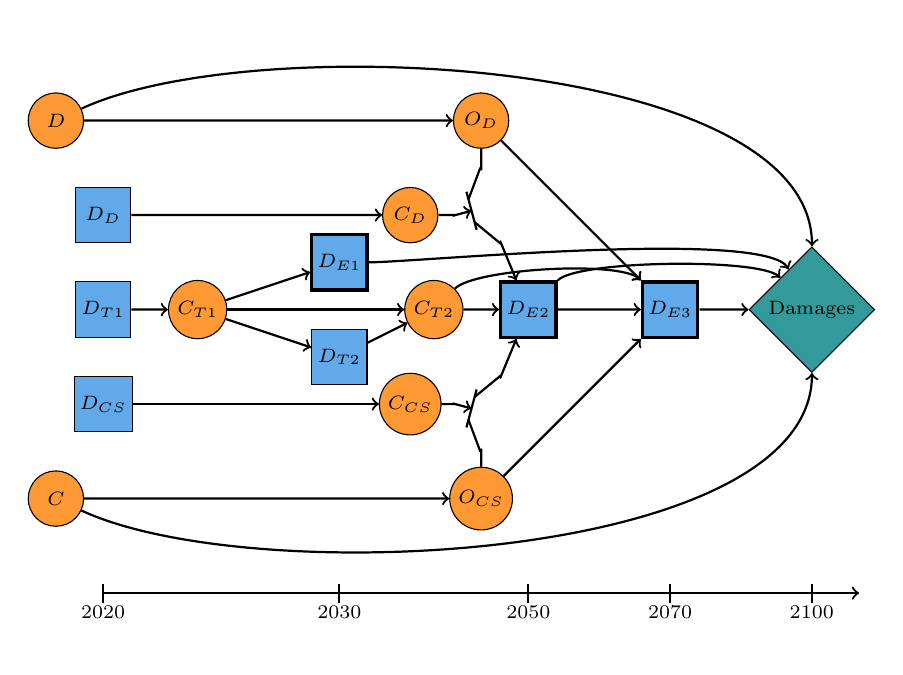
\begin{tikzpicture}
	    [decision/.style={fill=blue!80, draw, minimum size=2em, inner sep=2pt}, 
	    chance/.style={circle, fill=orange!80, draw, minimum size=2em, inner sep=2pt},
	    value/.style={diamond, fill=teal!80, draw, minimum size=2em, inner sep=2pt},
	    optimization/.style={ellipse, fill=teal!80, draw, minimum size=2em, inner sep=2pt},
	    scale=1.2, font=\scriptsize]
	     \node[decision] (D1) at (0, 2)   {$D_{D}$};
	     \node[decision] (D2) at (0, 1)   {$D_{T1}$};
	     \node[decision] (D3) at (0, 0)   {$D_{CS}$};
	     \node[decision, very thick] (D4) at (2.5, 1.5)   {$D_{E1}$};
	     \node[decision] (D5) at (2.5, 0.5)   {$D_{T2}$};
	     \node[decision, very thick] (D6) at (4.5, 1)   {$D_{E2}$};
	     \node[decision, very thick] (D7) at (6.0, 1)   {$D_{E3}$};
	     \node[chance]   (C0) at (-0.5, 3)  {$D$};
	     \node[chance]   (C00) at (-0.5, -1)  {$C$};
	     \node[chance]   (C1) at (3.25, 2)   {$C_{D}$};
	     \node[chance]   (C2) at (1, 1)   {$C_{T1}$};
	     \node[chance]   (C3) at (3.25, 0)   {$C_{CS}$};
	     \node[chance]   (C4) at (3.5, 1)   {$C_{T2}$};
	     \node[chance]   (O1) at (4, 3)   {$O_{D}$};
	     \node[chance]   (O2) at (4, -1)   {$O_{CS}$};
	     \draw[] (4.1,2.1) pic{dist_arc={int1, , ,rotate=105}};
	     \draw[] (4.1,-0.1) pic{dist_arc={int2, , ,rotate=75}};
	     \node[value] (SC) at (7.5, 1)   {Damages};
	     \draw[->, thick] (C0) -- (O1);
	     \draw[->, thick] (O1) -- (D7);
	     \draw[->, thick] (C0) to[out=25,in=90,distance=2cm] (SC);
	     \draw[->, thick] (C00) -- (O2);
	     \draw[->, thick] (O2) -- (D7);
	     \draw[->, thick] (C00) to[out=-25,in=-90,distance=2cm] (SC);
	     \draw[->, thick] (D1) -- (C1);
	     \draw[->, thick] (D2) -- (C2);
	     \draw[->, thick] (D3) -- (C3);
	    %  \draw[->, thick] (C1) -- (D4);
	    %  \draw[->, thick] (C1) -- (D5);
	     \draw[->, thick] (C2) -- (D4);
	     \draw[->, thick] (C2) -- (D5);
	     \draw[->, thick] (C2) -- (C4);
	    %  \draw[->, thick] (C3) -- (D4);
	    %  \draw[->, thick] (C3) -- (D5);
	     \draw[->, thick] (D5) -- (C4);
	    %  \draw[->, thick] (C2) -- (D6);
	     \draw[->, thick] (C4) -- (D6);
	     \draw[->, thick] (C4) to[out=45,in=135,distance=0.3cm] (D7);
	%     \draw[->, thick] (D4) to[out=0,in=90,distance=0.5cm] (D6);
	     \draw[->, thick] (D4) to[out=0,in=120,distance=0.5cm] (SC);
	     \draw[->, thick] (D6) -- (D7);
	     \draw[->, thick] (D6) to[out=45,in=135,distance=0.3cm] (SC);
	     \draw[->, thick] (D7) -- (SC);
	     \draw[thick] (C1) -- (int1.195);
	     \draw[thick] (O1) -- (int1.105);
	     \draw[->, thick] (int1.285) -- (D6);
	     \draw[thick] (C3) -- (int2.165);
	     \draw[thick] (O2) -- (int2.255);
	     \draw[->, thick] (int2.75) -- (D6);
	     \draw[->, thick] (0,-2) -- (8,-2);
	     \draw[-, thick] (0.0,-1.9) -- (0.0,-2.1);
	     \draw[-, thick] (2.5,-1.9) -- (2.5,-2.1);
	     \draw[-, thick] (4.5,-1.9) -- (4.5,-2.1);
	     \draw[-, thick] (6.0,-1.9) -- (6.0,-2.1);
	     \draw[-, thick] (7.5,-1.9) -- (7.5,-2.1);
	     \node[] at (0.0,-2.2) {2020};
	     \node[] at (2.5,-2.2) {2030};
	     \node[] at (4.5,-2.2) {2050};
	     \node[] at (6.0,-2.2) {2070};
	     \node[] at (7.5,-2.2) {2100};
	\end{tikzpicture}
	\end{figure}
\end{frame}



\begin{frame}{More recent developments}

	{\bf 2. Optimal information structures}
	\begin{itemize}
		\item We are interested in knowing \alert{what information} to acquire and \alert{when}
		\item Find optimal \alert{information structure} and \alert{decision strategy} 
	\end{itemize}
	
	We propose three alternative formulations:
	%
	\begin{enumerate}
		\item Constraints on path probabilities
		\item Constraints on local decisions
		\item Extended state space
	\end{enumerate}

\end{frame}

\begin{frame}{The extended pig farm problem} 

\begin{figure}[h]
\centering 
%\includegraphics[width = 0.6\textwidth]{./Figures/Figure_ExtendedCPP.JPG}
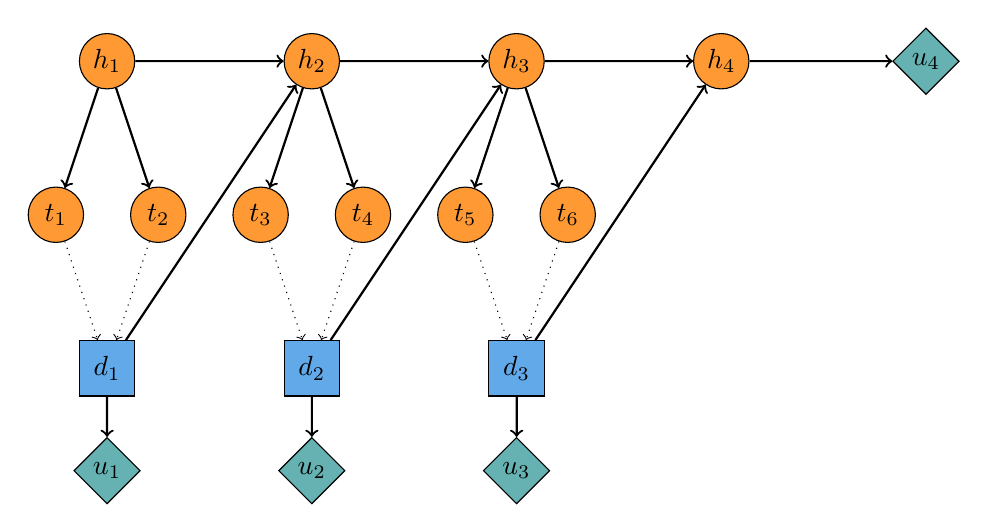
\begin{tikzpicture}
    [decision/.style={fill=blue!80, draw, minimum size=2em, inner sep=2pt}, 
    chance/.style={circle, fill=orange!80, draw, minimum size=2em, inner sep=2pt},
    value/.style={diamond, fill=teal!60, draw, minimum size=2em, inner sep=2pt},
    scale=1.3]
     %\draw[step=1cm,gray,very thin] (0,0) grid (4,3);
     \node[chance] (h1) at (0.5, 4)      {$h_1$};
     \node[chance] (h2) at (2.5, 4)      {$h_2$};
     \node[chance] (h3) at (4.5, 4)      {$h_3$};
     \node[chance] (h4) at (6.5, 4)      {$h_4$};
     \node[value]  (u4) at (8.5, 4)      {$u_4$};
     \node[chance] (t1) at (0, 2.5)      {$t_1$};
     \node[chance] (t2) at (1, 2.5)      {$t_2$};
     \node[chance] (t3) at (2, 2.5)      {$t_3$};
     \node[chance] (t4) at (3, 2.5)      {$t_4$};
     \node[chance] (t5) at (4, 2.5)      {$t_5$};
     \node[chance] (t6) at (5, 2.5)      {$t_6$};
     \node[decision] (d1) at (0.5, 1)    {$d_1$};
     \node[decision] (d2) at (2.5, 1)    {$d_2$};
     \node[decision] (d3) at (4.5, 1)    {$d_3$};
     \node[value] (u1) at (0.5, 0)       {$u_1$};
     \node[value] (u2) at (2.5, 0)       {$u_2$};
     \node[value] (u3) at (4.5, 0)       {$u_3$};
     \draw[->, thick] (h1) -- (t1);
     \draw[->, thick] (h1) -- (t2);
     \draw[->, thick] (h1) -- (h2);
     \draw[->, thick] (h2) -- (t3);
     \draw[->, thick] (h2) -- (t4);
     \draw[->, thick] (h2) -- (h3);
     \draw[->, thick] (h3) -- (t5);
     \draw[->, thick] (h3) -- (t6);
     \draw[->, thick] (h3) -- (h4);
     \draw[->, thick] (h4) -- (u4);
     \draw[->, dotted] (t1) -- (d1);
     \draw[->, dotted] (t2) -- (d1);
     %\draw[->, thick] (t1) -- (d2);
     %\draw[->, thick] (t1) -- (d3);
     \draw[->, dotted] (t3) -- (d2);
     \draw[->, dotted] (t4) -- (d2);
     %\draw[->, thick] (t2) -- (d3);
     \draw[->, dotted] (t5) -- (d3);
     \draw[->, dotted] (t6) -- (d3);
     %\draw[->, thick] (d1) -- (d2);
     \draw[->, thick] (d1) -- (h2);
     \draw[->, thick] (d1) -- (u1);
     \draw[->, thick] (d2) -- (h3);
     \draw[->, thick] (d2) -- (u2);
     %\draw[->, thick] (d2) -- (d3);
     %\draw[->, thick] (d1) -- (0.5, 0.5) -- (1.5,0.5) -- (d3);
     \draw[->, thick] (d3) -- (h4);
     \draw[->, thick] (d3) -- (u3);
\end{tikzpicture}
\end{figure}
	
\end{frame}


\begin{frame}{Better formulations}

New formulations: \alert{stronger formulations} in which we can replace indicator variables $\pi(s)$ with continuous variables.

\begin{figure}[ht]
\centering
     \begin{subfigure}[b]{0.48\textwidth}
         \centering
         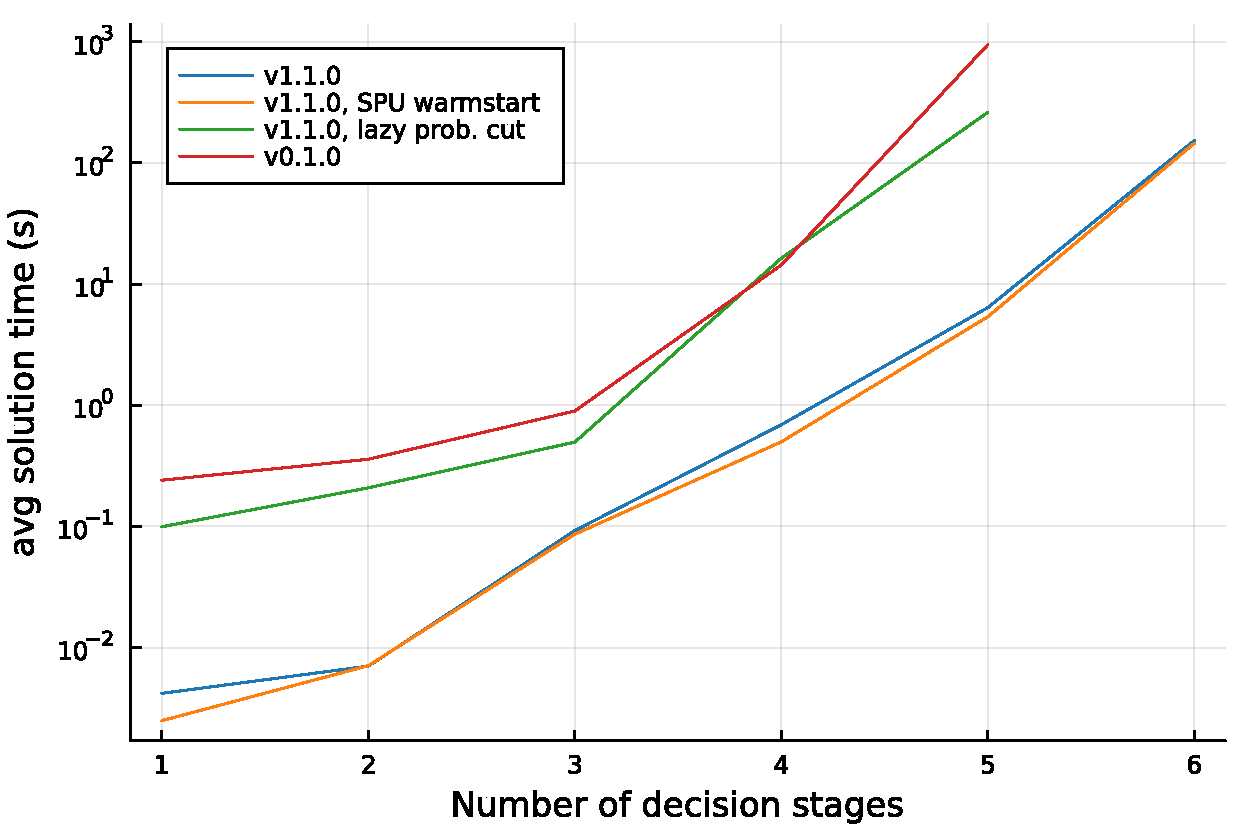
\includegraphics[width=\textwidth]{figures/sol_times_pigfarm.pdf}
         \caption{The pig farm problem}
         \label{fig:sol_times_pigfarm}
     \end{subfigure}
     \hfill
     \begin{subfigure}[b]{0.48\textwidth}
         \centering
         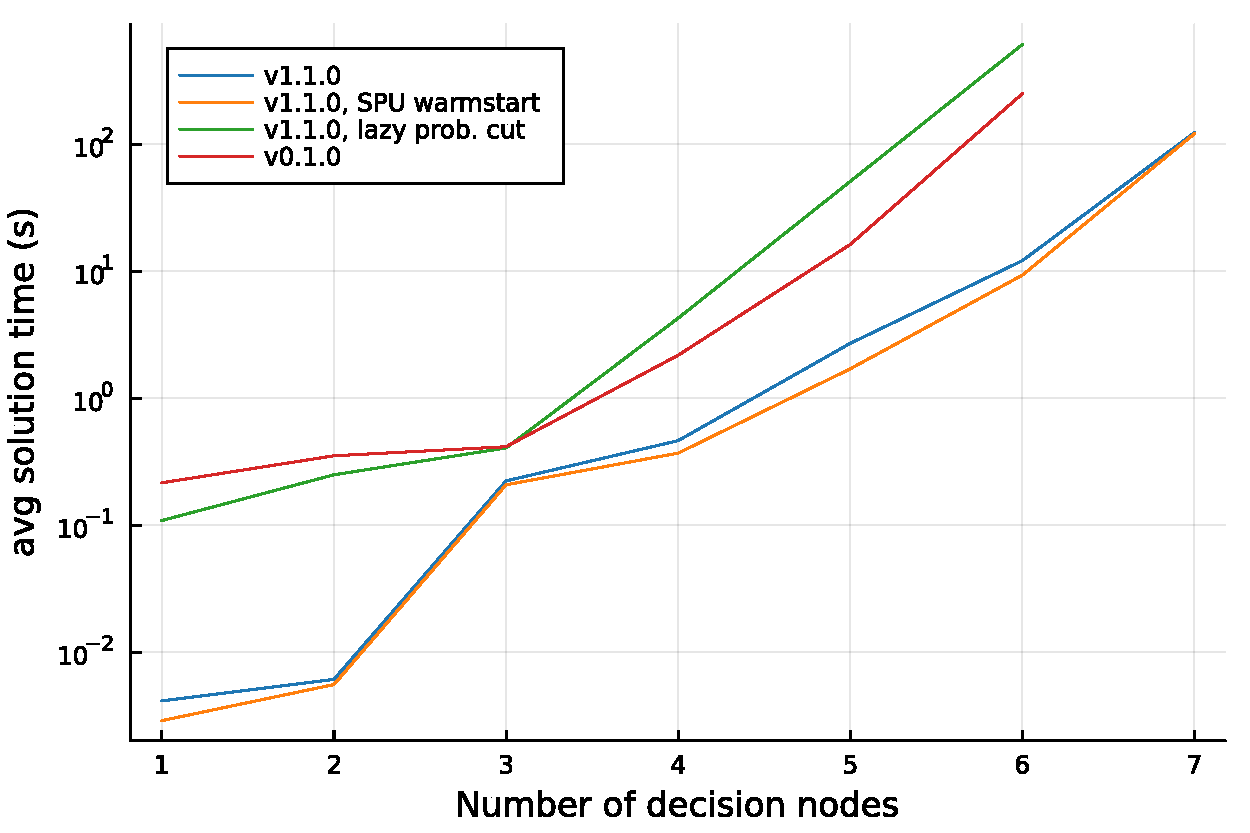
\includegraphics[width=\textwidth]{figures/sol_times_nmonitoring.pdf}
         \caption{The N-monitoring problem}
         \label{fig:sol_times_nmonitoring}
     \end{subfigure}
     \caption{The solution times of the two example problems with different number of decision nodes using different formulations. Notice the logarithmic y-axis.}
     \label{fig:sol_times}
\end{figure}
	
\end{frame}





\frame{
\thispagestyle{empty}
{\setlength{\parskip}{6pt}
\titlepage
}
}
  
\begin{frame}[allowframebreaks]{References}
\scriptsize
\bibliography{MyRef}
\bibliographystyle{apalike}


\end{frame}
  
    


\end{document}